
\chapter{Certificado autofirmado SSL}

Vamos a comenzar trabajando en m1, todos los comandos y configuraciones que se van a mostrar a continuación se ralizarán en esta máquina.

Primero creamos la carpeta donde vamos a guardar los certificados \verb|/etc/apache2/ssl| y luego vamos a activar el módulo ssl y relanzamos apache, para lo que ejecutamos los comandos que se muestran en \eqref{ssl_1}.

\begin{figure}[h!]
\begin{center}
\caption{Creación del directorio para almacenar los certificados, instalación del módulo ssl y relanzar apache.}
\label{ssl_1}
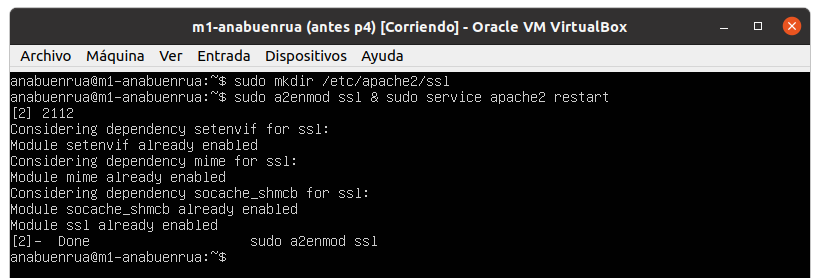
\includegraphics[scale=0.5]{ssl_1b}
\end{center}
\end{figure}

Ahora procedemos a crear los certificados con \verb|ssl|, como se ve en \eqref{ssl_3}.

\begin{figure}[h!]
\begin{center}
\caption{Creación de los certificados con ssl.}
\label{ssl_3}
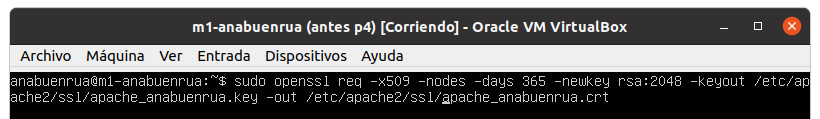
\includegraphics[scale=0.5]{ssl_3}
\end{center}
\end{figure}

En \eqref{ssl_3} hemos usado varios argumentos que explicamos a continuación:

\begin{itemize}
\item \verb|-x509|: Autofirma el certificado.
\item \verb|-days|: Indica que el certificado va a tener 365 días de validez.
\item \verb|-keyout|: Especifica el fichero donde se va a guardar la clave.
\item \verb|-out|: Especifica el fichero donde se va a guardar el certificado.
\end{itemize}

Además, le hemos indicado que la clave es de 2048 bits.

A continuación introducimos los datos que nos piden por línea de comandos, se ve en \eqref{ssl_4}.

\begin{figure}[h!]
\begin{center}
\caption{Introducimos los datos requeridos para la creación del certificado.}
\label{ssl_4}
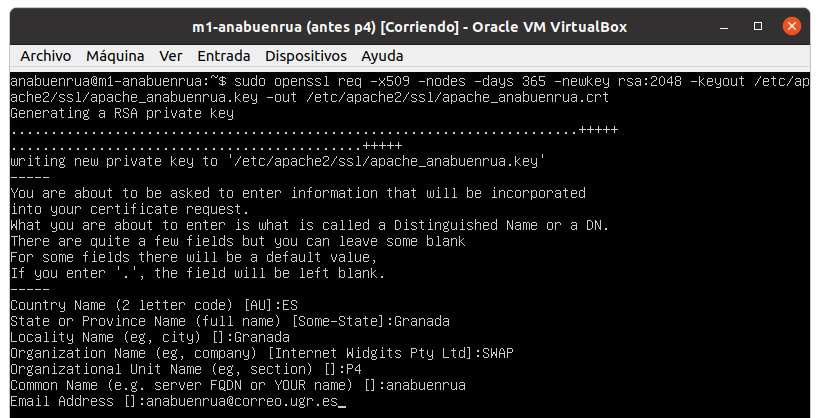
\includegraphics[scale=0.5]{ssl_4}
\end{center}
\end{figure}

\section{Opciones avanzadas}



\chapter{Apache con certificado SSL}



\section{Opciones avanzadas}



\chapter{Nginx como balanceador para peticiones HTTPS}



\section{Opciones avanzadas}



\chapter{IPTABLES}



\section{Configuración básica y abrir puertos}



\section{Opciones avanzadas}



\chapter{Configurar cortafuegos al arranque}

